
\section{Power markets}

See folders "`Electricity pricing"' and "`power markets"'

In this section different studies of power market characteristics are presented to distinguish features that may be used in building forecasting models. 

\subsection{Stable Modeling of different European Power Markets}

In this paper different European power markets have been investigated to reveal major differences in energy price behaviour \cite{mugele2005stable}. The EEX, Nord Pool Spot and Polish power markets have been evaluated whereby the markets are responsible for the Mid-Europe, Northern Europe and Polish regions respectively. 

As in general electricity prices depend on energy demand \cite{weron2005forecasting} which changes due to climate conditions (temperature and number of daylight hours) electricity prices exhibit a seasonal component as well (Figure \ref{fig:seasonal_behaviour_of_eex_prices}). 

\begin{figure}[htbp]
	\centering
		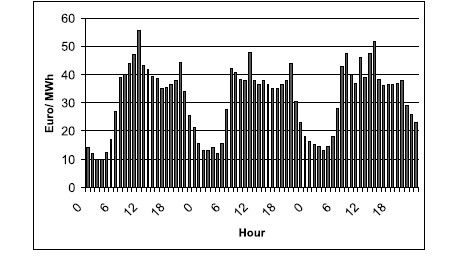
\includegraphics{figures/state_of_the_art/seasonal_behaviour_of_eex_prices.PNG}
	\caption{EEX - hourly spot prices \cite{mugele2005stable}}
	\label{fig:seasonal_behaviour_of_eex_prices}
\end{figure}

The main differences between electricity power markets and other financial markets are price volatility, mean reversion and price jumps or "`spikes"'. Volatility is high as generated electricity cannot be stored but has to be delivered at once which might lead to high prices on transmission congestion or surges in demand. It's impact can be reduced by applying logarithmic transformations of input data \cite{weron2005forecasting}. 

Energy prices experience strong mean reversion which denotes the characteristic that prices return to their mean levels after an increase in prices. In addition price spikes may appear where prices can increase tenfold from one hour to the next. To mitigate these spikes they may be averaged out in a data preprocessing step. 

Even though price seasonality and trend seem to be stable over a short time range (Figure \ref{fig:seasonal_behaviour_of_eex_prices}) they can show significant fluctuations over a longer time range. In \cite{mugele2005stable} data related to each examined energy market was fitted to a stable Paretian distribution as well as a normal distribution. The result showed that mature markets as EEX or Nord Pool Spot exhibit high volatility, heavy tails, high kurtosis and asymmetrics in the energy price data which was best modeled by the Paretian distribution. In contrast the Gielda Energii SA market in Poland shows a much more stable energy price behavior which can be modeled by a Gaussian distribution. 

The variation in energy price levels for the two power markets EEX and Nord Pool Spot are shown in Figures \ref{fig:EEX_levels} and \ref{fig:NordPool_levels}.

\begin{figure}[!htbp]
  \centering
  \begin{minipage}[b]{0.4\textwidth}
    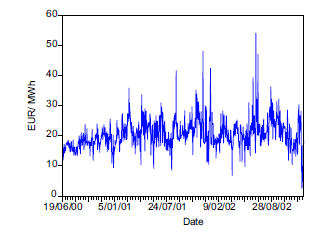
\includegraphics[width=\textwidth]{figures/state_of_the_art/EEX_levels.PNG}
    \caption{EEX levels \cite{mugele2005stable}}
		\label{fig:EEX_levels}
  \end{minipage}
  \hfill
  \begin{minipage}[b]{0.4\textwidth}
    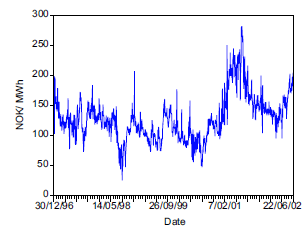
\includegraphics[width=\textwidth]{figures/state_of_the_art/NordPool_levels.PNG}
    \caption{Nord Pool levels \cite{mugele2005stable}}
		\label{fig:NordPool_levels}
  \end{minipage}
\end{figure}

This shows that it is important to investigate energy price characteristics from power markets to accurately model market prices. 




%
%\subsection{Electricity markets and pricing}
%
%In wholesale energy markets different pricing and bidding models can be used. Currently the two most common price evaluation strategies are day-ahead and real-time pricing strategies. 
%
%\subsubsection{Bidding strategies}
%
%In \cite{tierney2008uniform} two different bidding strategies are discussed, uniform pricing and pay-as-bid auctions. In the uniform pricing model the market clearing price is determined by collecting the marginal prices from all suppliers and taking the maximum price from this collection. Conversely, in pay-as-bid auctions a supplier gets paid based on its actual bid. 
%The second approach may seem beneficial from the customer's point of view since suppliers may set individual prices which enables competition within the market. 
%However studies show that in this pricing scheme suppliers set their prices at the maximum possible level to be comparable to other suppliers and keep their customers. On the other hand the uniform pricing model provides a uniform clearing price which is valid for all participants in the market and customers may trust that suppliers set prices to just satisfy their needs. 





%> locationId <- 1
%> simPrefix <- paste0("da_sim_",locationId,"_")
%>     type <- "DA"
%> simPostFix <- "_1w_1w"
%> sim2wRMSE <- getRMSEPerSimulation(paste0(simPrefix,"2w",simPostFix))
%> sim3wRMSE <- getRMSEPerSimulation(paste0(simPrefix,"3w",simPostFix))
%> sim4wRMSE <- getRMSEPerSimulation(paste0(simPrefix,"4w",simPostFix))
%> xtable(sim2wRMSE)
% latex table generated in R 3.1.1 by xtable 1.8-2 package
% Mon Mar 07 21:30:50 2016
\begin{table}[ht]
\centering
\begin{tabular}{rrrrrrrrrrr}
  \hline
 & 1h & 3h & 6h & 12h & 18h & 24h & 36h & 48h & 96h & 168h \\ 
  \hline
mean & 14.55 & 14.55 & 14.55 & 14.55 & 14.55 & 14.55 & 14.55 & 14.55 & 14.55 & 14.55 \\ 
  ses & 2.13 & 3.54 & 5.06 & 15.83 & 16.38 & 14.98 & 14.97 & 14.64 & 15.13 & 13.30 \\ 
  holts & 1.91 & 3.36 & 9.48 & 30.83 & 38.85 & 44.08 & 58.79 & 74.25 & 137.44 & 228.66 \\ 
  holtwinters & 3.20 & 7.11 & 13.10 & 26.07 & 36.13 & 45.85 & 65.02 & 85.30 & 166.43 & 288.31 \\ 
  arima & 2.11 & 3.06 & 4.63 & 13.68 & 13.92 & 12.69 & 12.88 & 12.62 & 13.69 & 12.97 \\ 
  tbats & 2.15 & 2.89 & 4.35 & 10.63 & 10.85 & 10.00 & 10.16 & 9.90 & 10.66 & 10.30 \\ 
   \hline
\end{tabular}
\end{table}
%> xtable(sim3wRMSE)
% latex table generated in R 3.1.1 by xtable 1.8-2 package
% Mon Mar 07 21:30:54 2016
\begin{table}[ht]
\centering
\begin{tabular}{rrrrrrrrrrr}
  \hline
 & 1h & 3h & 6h & 12h & 18h & 24h & 36h & 48h & 96h & 168h \\ 
  \hline
mean & 14.78 & 14.78 & 14.78 & 14.78 & 14.78 & 14.78 & 14.78 & 14.78 & 14.78 & 14.78 \\ 
  ses & 2.14 & 3.56 & 5.06 & 15.84 & 16.38 & 14.98 & 14.97 & 14.63 & 15.14 & 13.31 \\ 
  holts & 1.91 & 3.38 & 9.51 & 30.88 & 38.90 & 44.15 & 58.90 & 74.39 & 137.77 & 229.23 \\ 
  holtwinters & 3.08 & 7.08 & 13.15 & 27.16 & 37.14 & 46.56 & 65.62 & 85.74 & 166.63 & 288.04 \\ 
  arima & 2.06 & 2.88 & 4.31 & 12.94 & 13.08 & 11.89 & 11.97 & 11.66 & 12.71 & 11.79 \\ 
  tbats & 2.15 & 3.05 & 4.73 & 11.27 & 11.43 & 10.55 & 10.60 & 10.35 & 11.07 & 10.68 \\ 
   \hline
\end{tabular}
\end{table}
%> xtable(sim4wRMSE)
% latex table generated in R 3.1.1 by xtable 1.8-2 package
% Mon Mar 07 21:30:56 2016
\begin{table}[ht]
\centering
\begin{tabular}{rrrrrrrrrrr}
  \hline
 & 1h & 3h & 6h & 12h & 18h & 24h & 36h & 48h & 96h & 168h \\ 
  \hline
mean & 14.99 & 14.99 & 14.99 & 14.99 & 14.99 & 14.99 & 14.99 & 14.99 & 14.99 & 14.99 \\ 
  ses & 2.13 & 3.57 & 5.06 & 15.84 & 16.38 & 14.97 & 14.96 & 14.61 & 15.13 & 13.30 \\ 
  holts & 1.89 & 3.37 & 9.53 & 31.00 & 39.07 & 44.34 & 59.18 & 74.75 & 138.54 & 230.59 \\ 
  holtwinters & 5.52 & 11.00 & 17.21 & 33.23 & 44.51 & 54.36 & 75.54 & 97.71 & 187.49 & 324.07 \\ 
  arima & 1.98 & 2.85 & 4.39 & 12.68 & 12.79 & 11.61 & 11.73 & 11.36 & 12.07 & 11.13 \\ 
  tbats & 2.18 & 3.08 & 4.64 & 10.99 & 11.19 & 10.32 & 10.46 & 10.21 & 10.94 & 10.40 \\ 
   \hline
\end{tabular}
\end{table}



